\chapter{Generalized actions -ga}

	Suppose that there is a variable having two values $u_i, u_j$ and there are two actions that differs only in one thing. The difference is that one action has got $u_i$ in prevail precondition and the second has got $u_j$ in its prevail precondition. In such scenario, both actions can be generalized into one - the generalized action does not have any precondition on variable $\var{u_i}$. By this, we can reduce number of actions.


	\begin{figure}
		\begin{subfigure}[b]{0.8\textwidth}
			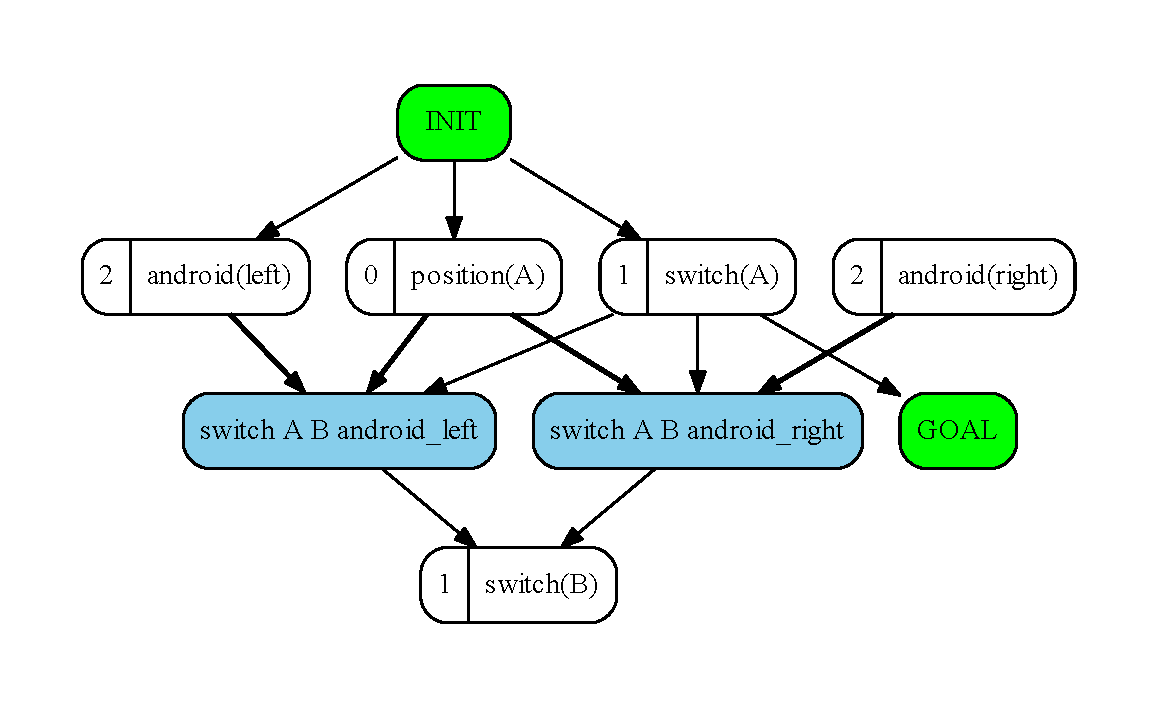
\includegraphics[scale=0.5]{generalizeActions/figures/simple_input}
			\caption{before reduction}
		\end{subfigure}	
		
		\begin{subfigure}[b]{0.8\textwidth}
			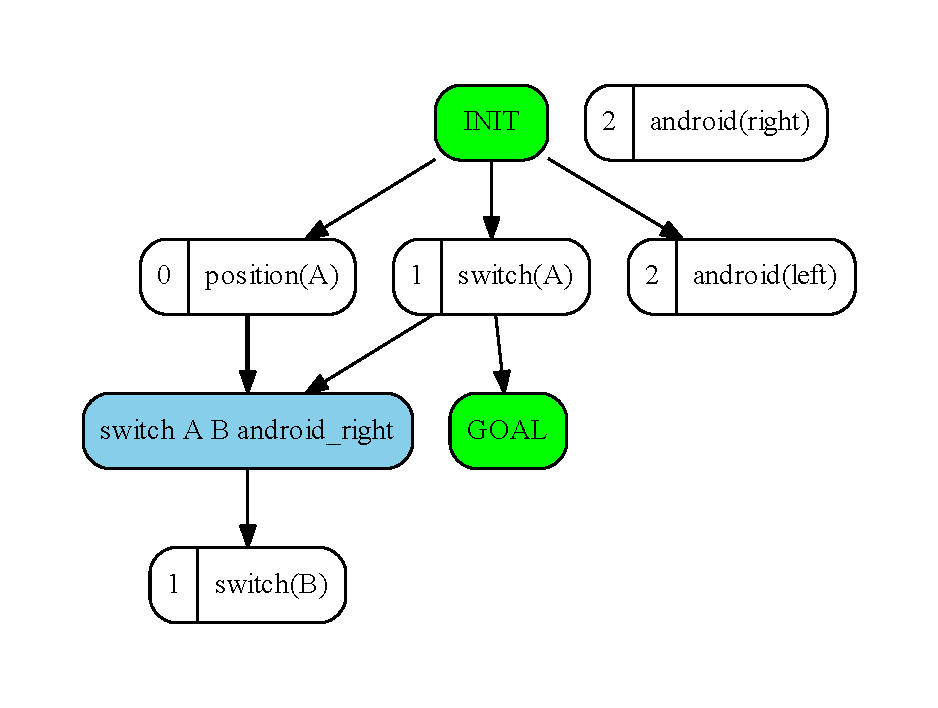
\includegraphics[scale=0.5]{generalizeActions/figures/simple_output}
			\caption{after reduction}
		\end{subfigure}
		\caption{Both action from the example can be generalized because their together cover all possibilities of variable 2 in preconditions. }
	\end{figure}               
	
	
	\section{Reduce operation}
	Let's have SAS in form $<\vars, \init, \goal, \actions, \mutexes{}>$. Suppose that we an action $a$. Then for each variable $v$ there exists set of actions $A_d$ that is created in this way: $\exists v \in \vars: A_v \leftarrow \{<\pre{a} \cup \{u\},\eff{a}> | \forall u \in \dom{v} \} $.
	
	If 	$A_v \subseteq \actions$ is satisfied for arbitrary $v$, then this operation can be executed. Then $a$ is generalized action thanks to variable $v$. 
	
	Now, the reduction can be executed as follow:
	
	\textbf{Case A)} $a \in \actions$
	$\actions{}' \leftarrow \actions \setminus A_s$
	
	\textbf{Case B)}
	$\actions{}' \leftarrow (\actions \setminus A_s) \cup \{a\}$
	
		
	Output of the reduction is SAS $<\vars{}, \init{}, \goal{}, \actions{}', \mutexes{}>$.
	
	
	\section{Possible outgoing states of SAS}
	\begin{enumerate}
		\item states of SAS where -mv, -bv, -uv, -mo, -sd, -hc can be executed, maybe also others
	\end{enumerate}
	
	\section{States before application of this operation}
	\begin{itemize}
		\item original SAS
		\item after execution of -dv, -mv
	\end{itemize}
	
	
	\section{Reverse operation}
	\textbf{Case A)} Removed actions are added back to SAS. No extension of the plan is done, because original SAS already contained generalized actions, so removed actions were redundant.
	
	\textbf{Case B)} Removed actions are added back to SAS. The plan is simulated and when action $a$ is used in the plan, it is replaced by corresponding action from $A_v$ having current value of variable $v$ in its prevail preconditions.
	
	
	\section{Implementation notes}
	Current implementation returns MultiReverseOperation.